\section{End-to-End Performance of Speculative Decoding}
\label{sect:e2e-perf}
In this section, we evaluate the performance of SD variants across various model sizes and datasets.
% The objective is to obtain a comprehensive view of its effectiveness in a real serving system.
The complete experimental setup is summarized in  \autoref{tab:exp-config} of the Appendix.
% \jerry{@Lily, I shifted it to Appendix.}

\subsection{Experiment Setup}
\textbf{Inference Engine and Hardware.}
All experiments are conducted using vLLM v0.10.1.1 unless otherwise stated.
To closely approximate real-world serving scenarios, we enable all default vLLM optimizations, 
including KV cache management, continuous batching, chunked prefill, and CUDA Graphs.
We run all experiments on NVIDIA H100~\cite{h100} with 80 GB of memory.
For 8B models, we use a single GPU, while for the 70B/106B models, we use four GPUs with a tensor parallel size of four. 
% \jerry{Citation}

\textbf{Models and SD variants}
We evaluate two models from the Llama-3 family \cite{dubey2024llama}:
Llama3.1-8B-Instruct and Llama3-70B-Instruct.
We also include Qwen3-8B\footnote{Throughout the paper, Qwen3-8B-Thinking denotes the same model with thinking mode enabled, whereas Qwen3-8B refers to its non-thinking mode.}~\cite{yang2025qwen3technicalreport} and GLM-4.5-Air-106B \cite{5team2025glm45agenticreasoningcoding} for reasoning workloads. We benchmark the following SD variants:
\begin{itemize} [leftmargin=1.5em, itemsep=0pt]
    \item \textbf{Draft-model-based}~\cite{leviathan2023fast, chen2023accelerating}: Uses a smaller draft model to propose 3 draft tokens per step, which are later verified by the target model. Details of model pairing are in Appendix~\autoref{appendix:model-config}.
  \item \textbf{EAGLE}~\cite{li2024eagle} and \textbf{EAGLE-3}~\cite{li2025eagle3}: Draft-model-free methods with fine-tuned auxiliary prediction heads, predicting 3 draft tokens per step for chain-based settings\footnote{Official EAGLE-3 weights are unavailable for Llama-3-70B, EAGLE weights are likewise unavailable for Qwen3-8B and EAGLE-3/EAGLE weights are also unavailable for GLM-4.5-Air~\cite{li2024eagle}.}.
  \item \textbf{Multi-Token Prediction} (MTP)~\cite{deepseekai2025deepseekv3technicalreport}: Co-trained draft-model-free approach where auxiliary heads are jointly trained with the target model; we use 3 draft tokens per step.
  \item \textbf{$n$-gram}~\cite{saxena2023prompt, somasundaram2024pld+}: Training-free method reusing recurring $n$-gram phrases from the prompt; we use 3 draft tokens per step with {\tt prompt\_lookup\_max=7} and {\tt prompt\_lookup\_min=3}. For \texttt{InstructCoder} with Llama3.1-8B, Llama3-70B and Qwen3-8B without reasoning, we additionally evaluate $n$-gram with 5 draft tokens per step to study the effect of a larger proposal length.
  
\end{itemize}
% \begin{itemize} [leftmargin=1.5em, itemsep=0pt]
%   \item \textbf{$n$-gram}~\cite{saxena2023prompt, somasundaram2024pld+}: 
%    5 draft tokens per step, with {\tt prompt\_lookup\_max=7} and {\tt prompt\_lookup\_min=3};
%   \item \textbf{EAGLE}~\cite{li2024eagle} and \textbf{EAGLE-3}~\cite{li2025eagle3} 3 draft tokens per step and the official draft models from the EAGLE authors.
%   \item \textbf{Draft-Model Based}~\cite{leviathan2023fast, chen2023accelerating}: 3 draft tokens per step.
%   \item \textbf{Multi-Token Prediction} (MTP)~\cite{deepseekai2025deepseekv3technicalreport}: 3 draft tokens per step. \jerry{Add specific eagle model used, smaller draft model used in appendix}
% \end{itemize}


Unless otherwise specified, the maximum generation length is capped at 8192 tokens.
For reasoning workloads AIME22-24 and GPQA-Main, we extend this limit to 32,768 tokens to prevent early truncation.
Decoding is performed with temperature set to 0 and no sampling truncation (\texttt{top\_p=1}, \texttt{top\_k=-1}).
% to minimize differences in output lengths across different methods.

\textbf{Workloads.}
We evaluate six datasets representing diverse real-world applications:
\textit{CNN/DailyMail}~\cite{hermann2015teaching, see-etal-2017-get} (summarization),
\textit{ShareGPT}~\cite{sharegpt} (multi-turn chat),
\textit{InstructCoder}~\cite{li2024instructcoder} (code editting),
\textit{GSM8K}~\cite{cobbe2021gsm8k} (grade-school math),
and two complex reasoning datasets: \textit{AIME22-24}~\cite{AIME-AoPS, AIME-HF} and \textit{GPQA-Main}~\cite{rein2023gpqagraduatelevelgoogleproofqa}. We detailed the dataset information in Appendix \autoref{appendix:dataset}. 
% \jerry{Add more description;}


% For each dataset, we randomly sample up to \textbf{500} requests (or the dataset maximum if smaller). To emulate different system loads, we vary the batch size from 1 to 128 requests during inference. Reasoning workloads use smaller batch sizes from 1 to 4 due to their longer generation lengths. Figure~\ref{fig:dataset} shows the input and output length distributions for all datasets using Qwen3-8B after filtering. \jerry{TODO: readers wont know what filtering means here}.

% \begin{figure}[t]
%     \centering
%     \begin{subfigure}[b]{\columnwidth}
%         \centering
%         \includegraphics[width=\linewidth]{figures/workload_length_distribution/after_filtering/input_length_distributions_Qwen3-8B.pdf}
%         \caption{Input length distributions.}
%         \label{fig:data-input}
%     \end{subfigure}
%     \begin{subfigure}[b]{\columnwidth}
%         \centering
%         \includegraphics[width=\linewidth]{figures/workload_length_distribution/after_filtering/output_length_distributions_Qwen3-8B.pdf}
%         \caption{Output length distributions.}
%         \label{fig:data-output}
%     \end{subfigure}

%     \caption{Dataset input and output length distributions. \lily{change tick to 5K, 10K...}}
%     \label{fig:dataset}
% \end{figure}
% \jerry{TODO: check with Lily on which figure to use for input/output length figure, add citations for datasets}


\textbf{Generation Length and Evaluation Metrics.}
Although in theory SD should preserve the same token distribution as standard decoding, in practice we observe discrepancies in the generated outputs—-{\em even under greedy decoding.} \autoref{tab:gen-len} illustrates this by showing variations in generation length when using the same set of prompts while changing the batch size and SD variant.
For each configuration, we replicate each request multiple times to match the target batch size.
We repeat the process for 500 requests and record the generation length for each request.
\begin{table}[h]
\centering
\caption{Average generation length (mean $\pm$ standard deviation) of the baseline (w/o SD) and different SD variants on the ShareGPT dataset using Llama3.1-8B across varying batch sizes.}
\label{tab:gen-len}
\resizebox{0.9\linewidth}{!}{
\begin{tabular}{ccccc}
\hline
\textbf{Batch Size} & \textbf{w/o SD} & \textbf{ngram} & \textbf{Eagle} & \textbf{Eagle3} \\
\hline
1   & 737$\pm$1048 & 750$\pm$1100 & 731$\pm$1010 & 736$\pm$1046 \\
8   & 722$\pm$994  & 676$\pm$810  & 709$\pm$928  & 704$\pm$916  \\
16  & 708$\pm$932  & 675$\pm$818  & 686$\pm$853  & 686$\pm$853  \\
32  & 674$\pm$784  & 697$\pm$887  & 693$\pm$857  & 706$\pm$917  \\
64  & 687$\pm$852  & 696$\pm$911  & 709$\pm$924  & 709$\pm$924  \\
128 & 714$\pm$930  & 739$\pm$1050 & 709$\pm$924  & 709$\pm$924  \\
\hline
\end{tabular}
}
\end{table}

As shown in \autoref{tab:gen-len}, even without speculative decoding (the w/o SD column), generation length differs across different batch sizes, and similarly when SD is used. Importantly, these differences are not consistently longer or shorter than the baseline, suggesting that they stem from numerical nondeterminism rather than implementation bugs.
Recent work~\cite{he2025nondeterminism} attributes such variability to kernel-level nondeterminism and floating-point variation during GPU execution.

To account for fluctuations in output length, we use token \textbf{throughput}, i.e., the number of generated tokens per second, as the performance metric.
This measure removes the confounding effect of varying generation lengths. \textbf{Speedup} is then defined as the ratio between the throughput with speculative decoding (SD) and the throughput without it.

% Our primary evaluation metric is the \textbf{average end-to-end request latency}, measured from request arrival to completion.
% We compare this latency against standard (non-SD) decoding under identical configurations and report the resulting speedup ratio.
% Each configuration (model, dataset, SD variant, and batch size) is executed once after a short warmup phase.

\subsection{Results}
\begin{figure*}[h!]
\begin{center}
\captionsetup{justification=centering}

\includegraphics[width=0.6\linewidth]{figures/e2e/legend.pdf}
  
\begin{subfigure}[t]{0.22\textwidth}
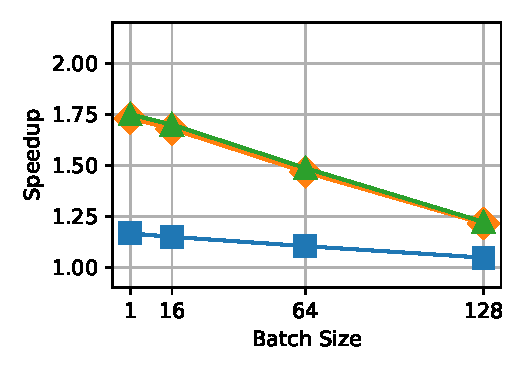
\includegraphics[width=\linewidth]{figures/e2e/gen_speedup_llama3-8b_gsm8k.pdf}
\caption{Llama3.1-8B, GSM8K}
\end{subfigure}
\begin{subfigure}[t]{0.22\textwidth}
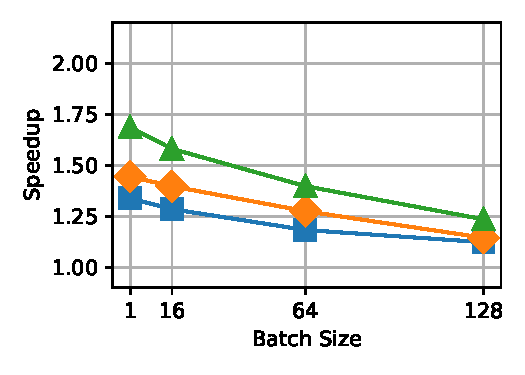
\includegraphics[width=\linewidth]{figures/e2e/gen_speedup_llama3-8b_cnndailymail.pdf}
\caption{Llama3.1-8B, CNN/Dailymail}
\end{subfigure}
\begin{subfigure}[t]{0.22\textwidth}
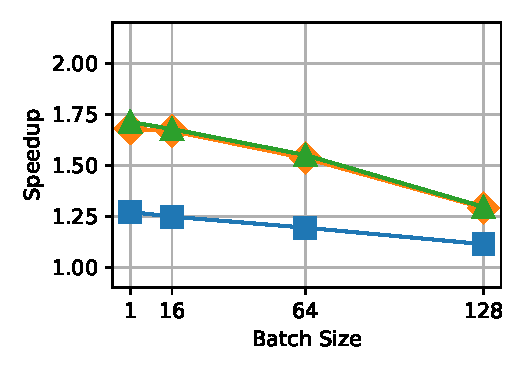
\includegraphics[width=\linewidth]{figures/e2e/gen_speedup_llama3-8b_sharegpt.pdf}
\caption{Llama3.1-8B, ShareGPT}
\end{subfigure}
\begin{subfigure}[t]{0.22\textwidth}
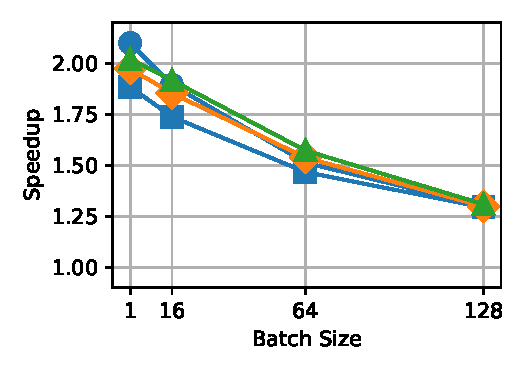
\includegraphics[width=\linewidth]{figures/e2e/gen_speedup_llama3-8b_instructcoder.pdf}
\caption{Llama3.1-8B, InstructCoder}
\end{subfigure}

\begin{subfigure}[t]{0.22\textwidth}
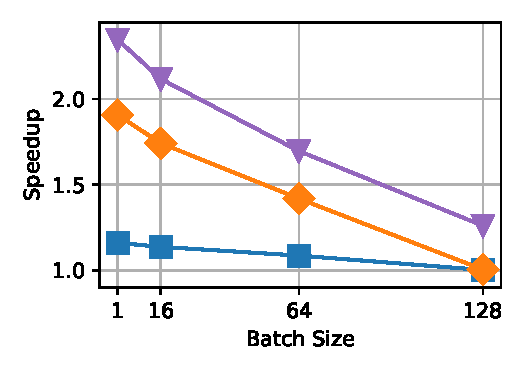
\includegraphics[width=\linewidth]{figures/e2e/gen_speedup_llama3-70b_gsm8k.pdf}
\caption{Llama3-70B, GSM8K}
\end{subfigure}
\begin{subfigure}[t]{0.22\textwidth}
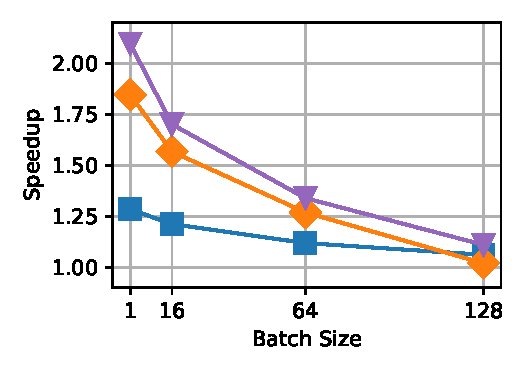
\includegraphics[width=\linewidth]{figures/e2e/gen_speedup_llama3-70b_cnndailymail.pdf}
\caption{Llama3-70B, CNN/Dailymail}
\end{subfigure}
\begin{subfigure}[t]{0.22\textwidth}
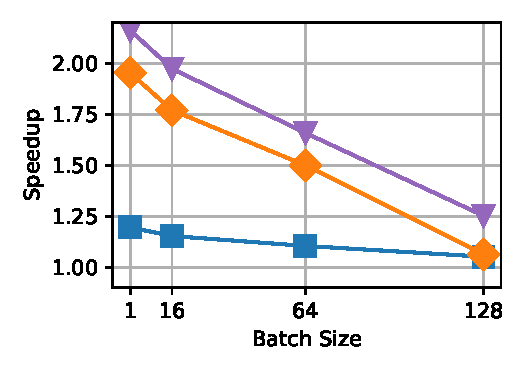
\includegraphics[width=\linewidth]{figures/e2e/gen_speedup_llama3-70b_sharegpt.pdf}
\caption{Llama3-70B, ShareGPT}
\end{subfigure}
\begin{subfigure}[t]{0.22\textwidth}
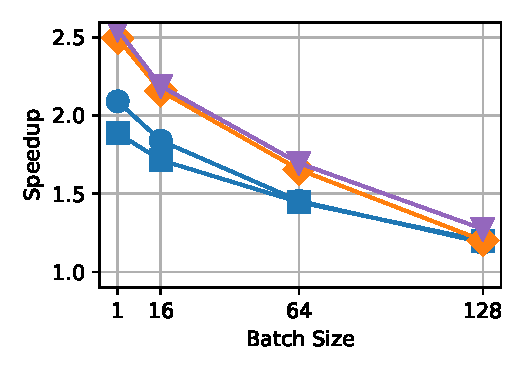
\includegraphics[width=\linewidth]{figures/e2e/gen_speedup_llama3-70b_instructcoder.pdf}
\caption{Llama3-70B, InstructCoder}
\end{subfigure}

\begin{subfigure}[t]{0.22\textwidth}
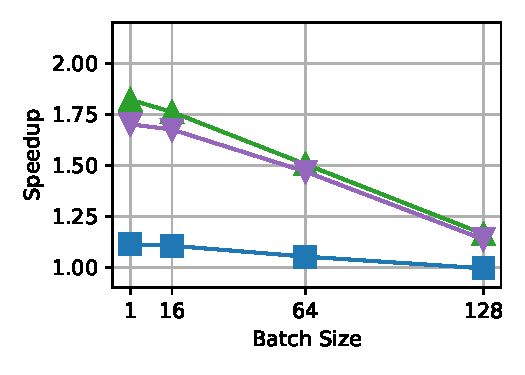
\includegraphics[width=\linewidth]{figures/e2e/gen_speedup_qwen-8b-no-thinking_gsm8k.pdf}
\caption{Qwen3-8B, GSM8K}
\end{subfigure}
\begin{subfigure}[t]{0.22\textwidth}
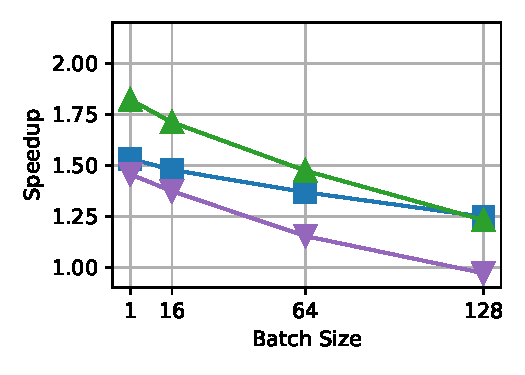
\includegraphics[width=\linewidth]{figures/e2e/gen_speedup_qwen-8b-no-thinking_cnndailymail.pdf}
\caption{Qwen3-8B, CNN/Dailymail}
\end{subfigure}
\begin{subfigure}[t]{0.22\textwidth}
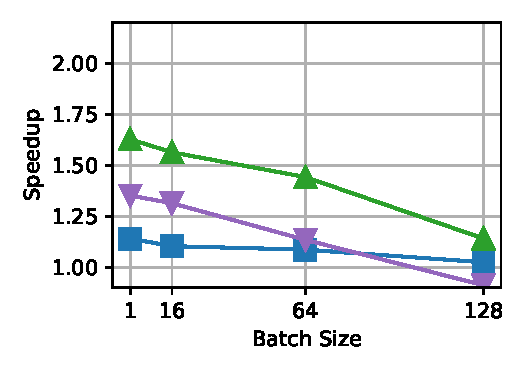
\includegraphics[width=\linewidth]{figures/e2e/gen_speedup_qwen-8b-no-thinking_sharegpt.pdf}
\caption{Qwen3-8B, ShareGPT}
\end{subfigure}
\begin{subfigure}[t]{0.22\textwidth}
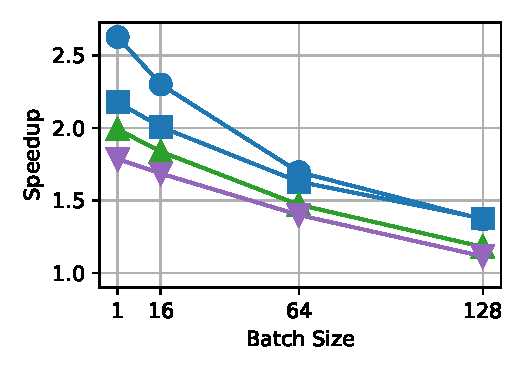
\includegraphics[width=\linewidth]{figures/e2e/gen_speedup_qwen-8b-no-thinking_instructcoder.pdf}
\caption{Qwen3-8B, InstructCoder}
\end{subfigure}

\caption{End-to-end performance on non-reasoning workloads. For the $n$-gram method, we report results for both three-token and five-token proposals.}
\label{fig:e2e-speedup}
\end{center}
\end{figure*}

\textbf{End-to-end speedup.} We first present the end-to-end throughput comparison in \autoref{fig:e2e-speedup}.
Across most configurations, SD improves throughput over the baseline without SD. The improvement is most pronounced with small/medium
batch sizes, when the system is memory-bound, so lots of compute can be used for proposing and verification.


\begin{quoting}[leftmargin=1.5em, rightmargin=1.5em, vskip=0pt]
\textbf{Batch Size.}
\emph{Increasing batch size improves absolute throughput but systematically reduces the relative speedup of speculative decoding, an effect that is amplified for larger models.}
\end{quoting}

Consistent with prior work~\cite{liu2024dsd}, larger batch sizes yield higher absolute throughput but lower relative speedup. For example, for the Llama3.1-8B model on the GSM8K dataset, the speedup of EAGLE over the non-SD baseline decreases from 1.73$\times$ to 1.21$\times$ as the batch size increases from 1 to 128.

At a high level, SD trades additional computation for increased throughput or reduced latency. When the batch size is small, the system has sufficient idle compute resources, so the extra computation-spent on proposing and verifying tokens that are ultimately rejected—has limited impact. However, as the batch size grows, the system becomes increasingly compute-bound, making the overhead spent on proposing and verifying rejected tokens more costly, and thus leading to smaller speedups. As shown in \autoref{sec:breakdown}, the verification stage dominates the overall execution time under such conditions.

We further observe that this trade-off between computation and speedup becomes more obvious as the model size increases. For instance, with EAGLE, on the ShareGPT dataset, increasing the batch size from 1 to 32 reduces the speedup by 4.3\% (1.68$\times$ to 1.61$\times$) for Llama3.1-8B, whereas for Llama3-70B, the speedup drops by 14.0\% (1.96$\times$ to 1.72$\times$). This trend arises because the 70B model is executed on four GPUs, so even with small or medium batch sizes, the system is already compute-bound, leaving limited spare compute to verify tokens that are ultimately rejected.


\begin{quoting}[leftmargin=1.5em, rightmargin=1.5em, vskip=0pt]
\textbf{SD Variants and dataset.}
\emph{
The $n$-gram method is generally less effective than other SD approaches across most workloads, with the notable exception of code-editing tasks. Moreover, the draft-model-based method achieves the best performance on the 70B target model; however, the effectiveness diminishes as the target model size decreases (e.g., 8B).}
\end{quoting}
GSM8K, CNN/DailyMail, and ShareGPT all show similar trends, with EAGLE-3 or draft-model-based method achieving the highest speedup across batch sizes. 
In contrast, on InstructCoder, the performance gap among SD variants narrows. For both Llama3.1-8B and Qwen3-8B, the $n$-gram method even outperforms EAGLE and EAGLE-3. This behavior arises because code-editing workloads such as InstructCoder exhibit strong token reuse, which can be effectively exploited by simple drafting methods like $n$-gram.
We further analyze the performance of $n$-gram in \autoref{subsect:ngram-bleu-score}.

% \jerry{NOTE: I updated the data for 70B draft model.}

% Next, we observe that draft-model-based methods achieve performance comparable to EAGLE on the Llama3-70B model, whereas on Qwen3-8B their performance is consistently worse than EAGLE-3 and, in some cases, even worse than $n$-gram. 
Next, we observe that draft-model–based methods outperform EAGLE on the Llama3-70B model in most settings. As shown in \autoref{fig:acc-len-request-level-box-plot}, draft-model–based approaches achieve higher token acceptance rates, while their proposing overhead is comparable to that of EAGLE (see \autoref{fig:exec-breakdown}). This behavior is expected: draft models are pretrained on large-scale corpora, whereas the EAGLE head is only fine-tuned on a relatively limited dataset, which naturally constrains its acceptance rate.

In contrast, on Qwen3-8B, draft-model–based speculative decoding consistently underperforms EAGLE-3 and, in some cases, even the training-free $n$-gram method.
% This degradation is primarily driven by the higher proposing overhead of draft-model–based SD on smaller target models. 
Specifically, for Llama3-70B, we use Llama3.2-1B as the draft model, whereas for Qwen3-8B we use Qwen3-0.6B. Although acceptance rates can be similar across the 70B and 8B setups on the same dataset—or even higher for the 8B case sometimes—draft-model–based SD is nonetheless noticeably less effective on the smaller model. For example, on GSM8K, the acceptance rate is 75\% for the 70B setup and 81\% for the 8B setup, yet the overall performance gain is substantially lower for Qwen3-8B.

This discrepancy arises because the proposing overhead is substantially larger for the 8B model. Specifically, the execution-time ratio between the draft and target model's single forward pass is around 12.5\% for the 70B setup, compared to an estimated 37.5\% for the 8B setup. As a result, drafting becomes significantly more expensive relative to verification on smaller models, which diminishes the overall benefit of draft-model-based SD.

% \jerry{(Hmm, the acceptance rate can be different for different datasets; for example, on GSM8K, it is 55\% for 70B and 80\% for 8B -\>, thus we see draft-model has similar performance on GSM8K for 70B and 8B; For ShareGPT, 53\% for 70B v.s. 60\% for 8B.}, 



% \jerry{We also find that draft-model-based SD maintains similar speedup as EAGLE for Llama3-70B, but its speedup is lower than EAGLE3 for Qwen3-8B.  
% [JERRY-TODO] due to limited choice of draft model, parameter size ratio -> also, drafting overheads; acceptance rates}
% For Llama3-70B on GSM8K, EAGLE’s speedup drops from 1.90$\times$ to 1.00$\times$, while draft-model-based SD declines more gradually from 1.86$\times$ to 1.39$\times$. This can be attributed to its higher average acceptance rate (0.55 versus 0.45 for EAGLE), particularly beneficial at large batch sizes where the verification phase dominates execution time and the system becomes compute-bound.}
% \jerry{@Lily But acceptance rate for draft-model is 1.21x higher but speedup is 1.39x higher. It could be EAGLE's 0.45 acc rate is not very accurate; this is from a quick run over 50 requests.}

% \jerry{We also find that the draft-model-based method maintains similar speedup as EAGLE for Llama3-70B, but its speedup is lower than EAGLE3 for Qwen3-8B. }

% Figures
\begin{figure*}[h!]
\begin{center}
\captionsetup{justification=centering}

\includegraphics[width=0.8\linewidth]{figures/e2e/draft-tree-500reqs/legend.pdf}

\begin{subfigure}[t]{0.22\textwidth}
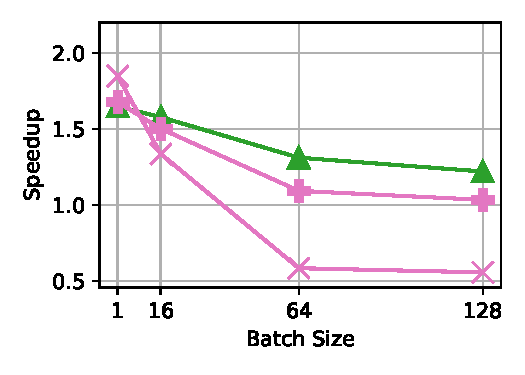
\includegraphics[width=\linewidth]{figures/e2e/draft-tree-500reqs/q3-8b/sglang-only_gsm8k.pdf}
\caption{Qwen3-8B, GSM8K}
\end{subfigure}
\begin{subfigure}[t]{0.22\textwidth}
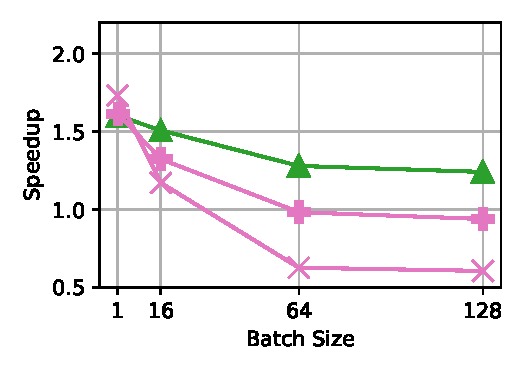
\includegraphics[width=\linewidth]{figures/e2e/draft-tree-500reqs/q3-8b/sglang-only_cnndailymail.pdf}
\caption{Qwen3-8B, CNN/Dailymail}
\end{subfigure}
\begin{subfigure}[t]{0.22\textwidth}
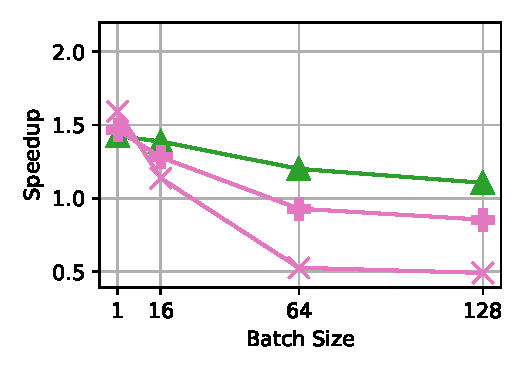
\includegraphics[width=\linewidth]{figures/e2e/draft-tree-500reqs/q3-8b/sglang-only_sharegpt.pdf}
\caption{Qwen3-8B, ShareGPT}
\end{subfigure}
\begin{subfigure}[t]{0.22\textwidth}
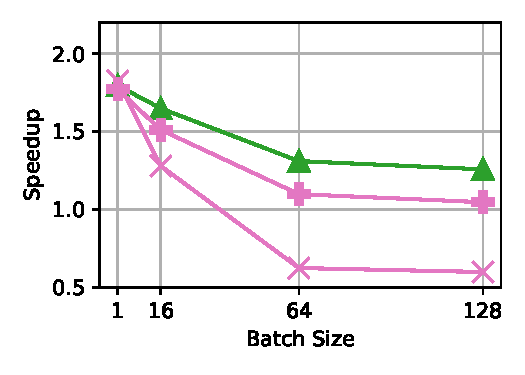
\includegraphics[width=\linewidth]{figures/e2e/draft-tree-500reqs/q3-8b/sglang-only_instructcoder.pdf}
\caption{Qwen3-8B, InstructCoder}
\end{subfigure}

% L3-70B
\begin{subfigure}[t]{0.22\textwidth}
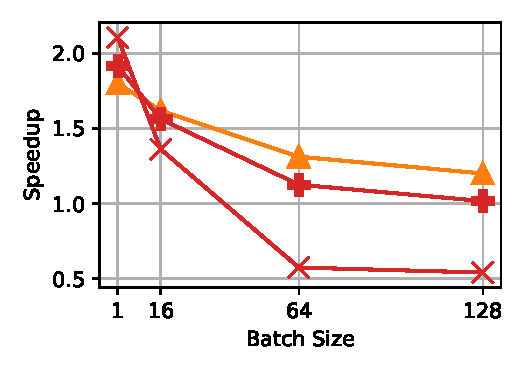
\includegraphics[width=\linewidth]{figures/e2e/draft-tree-500reqs/l3-70b/sglang-only_gsm8k.pdf}
\caption{Llama3-70B, GSM8K}
\end{subfigure}
\begin{subfigure}[t]{0.22\textwidth}
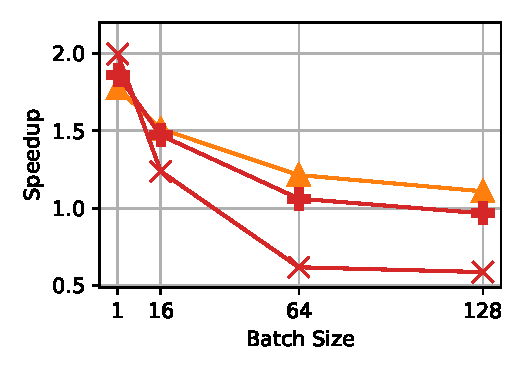
\includegraphics[width=\linewidth]{figures/e2e/draft-tree-500reqs/l3-70b/sglang-only_cnndailymail.pdf}
\caption{Llama3-70B, CNN/Dailymail}
\end{subfigure}
\begin{subfigure}[t]{0.22\textwidth}
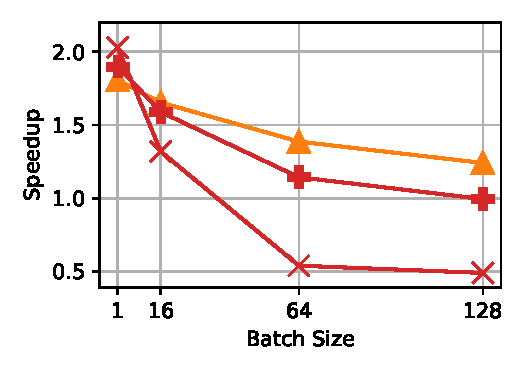
\includegraphics[width=\linewidth]{figures/e2e/draft-tree-500reqs/l3-70b/sglang-only_sharegpt.pdf}
\caption{Llama3-70B, ShareGPT}
\end{subfigure}
\begin{subfigure}[t]{0.22\textwidth}
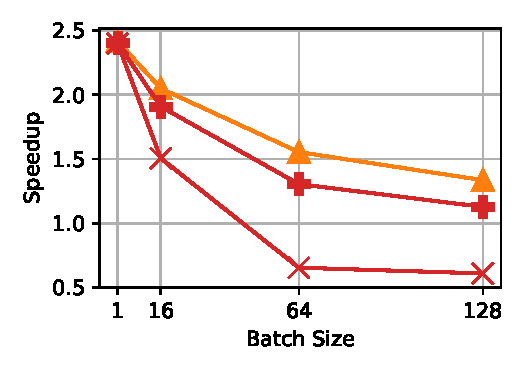
\includegraphics[width=\linewidth]{figures/e2e/draft-tree-500reqs/l3-70b/sglang-only_instructcoder.pdf}
\caption{Llama3-70B, InstructCoder}
\end{subfigure}
\caption{End-to-end performance on non-reasoning workloads for tree-style verification. We compare a chain setting ($k{=}3$) against tree settings with $k{=}6$ and $k{=}21$, using a fixed depth of 3 for all runs.}
\label{fig:e2e-speedup-tree}
\end{center}
\end{figure*}

\begin{quoting}[leftmargin=1.5em, rightmargin=1.5em, vskip=0pt]
\textbf{Tree-Style Verification.}
\emph{Tree-based methods provide slightly higher speedup at batch size 1, but the advantage quickly disappears as batch size increases. Across batch sizes, the chain-style method often remains the more performant.}
\end{quoting}

% We study tree-style verification in SGLang v0.5.9~\cite{zheng2024sglang} using Qwen3-8B and Llama3-70B on the non-reasoning workloads. We use SGLang here because the current vLLM draft-tree path we tested is not yet fully optimized, making it difficult to compare tree settings fairly. To keep the comparison controlled, we fix the tree depth to 3 in all runs. We use the chain setting with $k{=}3$ as the baseline, evaluate $k{=}21$ with a branching factor of 4 to roughly match the tree structure used in the EAGLE paper~\cite{li2024eagle}, and include $k{=}6$ with a branching factor of 2 as a smaller intermediate tree. Here, $k$ denotes the number of draft tokens verified in parallel by the target model. Unless otherwise noted, we use the same experimental settings as described earlier. By default, SGLang enables a dynamic draft-tree policy that adjusts the tree structure during decoding~\cite{li2024eagle}. Also, FlashAttention3~\cite{shah2024flashattention} is used for the chain case, while FlashInfer~\cite{ye2025flashinfer} is used for the tree cases by default.

We next evaluate tree-style verification in SGLang v0.5.9~\cite{zheng2024sglang} using Qwen3-8B and Llama3-70B on the non-reasoning workloads. We use SGLang for this study because the draft-tree path in the vLLM version we evaluated is not yet sufficiently optimized for a fair comparison across tree configurations. To control the comparison, we fix the tree depth to 3 in all runs. We use chain-style verification with $k{=}3$ as the baseline, evaluate a wider tree with $k{=}21$ and branching factor 4 to approximately match the tree structure used in EAGLE~\cite{li2024eagle}, and include an intermediate tree with $k{=}6$ and branching factor 2. Here, $k$ denotes the number of draft tokens verified in parallel by the target model. Unless otherwise noted, all other settings follow those described earlier. By default, SGLang uses a dynamic draft-tree policy which optimises the tree structure during decoding~\cite{li2024eagle}. In this setup, FlashAttention-3~\cite{shah2024flashattention} is used for the chain configuration, whereas FlashInfer~\cite{ye2025flashinfer} is used for the tree configurations.

As shown in \autoref{fig:e2e-speedup-tree}, tree-based EAGLE/EAGLE-3 achieves slightly higher speedup than the chain-based settings at batch size 1. For example, on Qwen3-8B with GSM8K, speedup increases from 1.65$\times$ for the chain to 1.68$\times$ for $k{=}6$ and 1.85$\times$ for $k{=}21$. On Llama3-70B with ShareGPT, it rises from 1.81$\times$ to 1.90$\times$ and 2.03$\times$. However, this benefit quickly disappears as batch size increases. By batch size 64, the $k{=}21$ tree falls below 1$\times$ speedup on all workloads for both models, whereas the chain remains above 1$\times$ throughout.

This is likely because wider trees increase the accepted length, but also verify many more tokens that are later rejected. On Qwen3-8B with GSM8K, the accepted length increases from 2.25 for the chain to 2.51 and 2.92 for the $k{=}6$ and $k{=}21$ trees, respectively, while the acceptance rate decreases from 0.415 to 0.300 and 0.095. We observe the same trend on Llama3-70B with ShareGPT (accepted length: 2.29 $\rightarrow$ 2.55 $\rightarrow$ 2.93; acceptance rate: 0.429 $\rightarrow$ 0.310 $\rightarrow$ 0.097). As discussed in \autoref{sec:breakdown}, verification dominates the execution cost, so the overhead of these additional rejected branches becomes increasingly expensive at larger batch sizes. Thus, tree-style verification provides only a narrow low-batch-size benefit, while chain-style verification remains the more robust setting overall.

\begin{figure*}[h!]
\captionsetup{justification=centering}
\begin{center}
\begin{subfigure}[t]{0.22\textwidth}
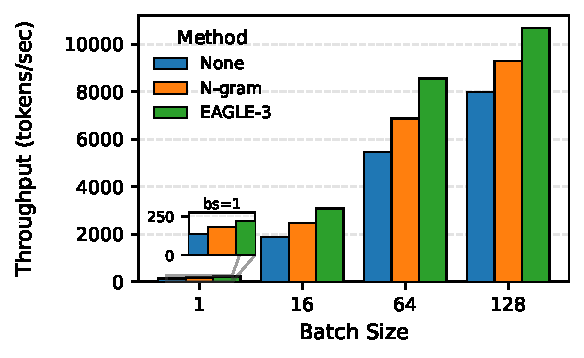
\includegraphics[width=\linewidth]{figures/e2e/thinking_qwen-8b-thinking_gsm8k.pdf}
\caption{Qwen3-8B-Thinking, GSM8K}
\end{subfigure}
\begin{subfigure}[t]{0.22\textwidth}
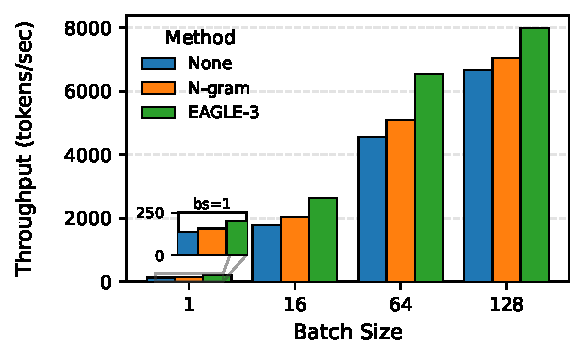
\includegraphics[width=\linewidth]{figures/e2e/thinking_qwen-8b-thinking_cnndailymail.pdf}
\caption{Qwen3-8B-Thinking, CNN/Dailymail}
\end{subfigure}
\begin{subfigure}[t]{0.22\textwidth}
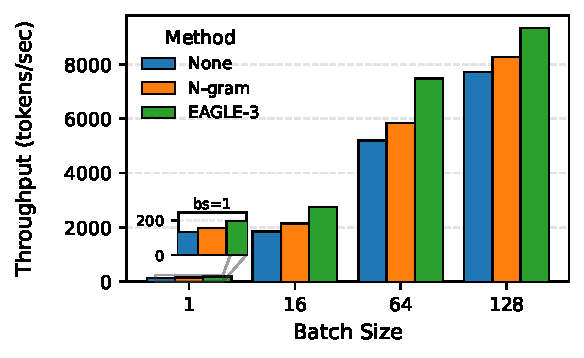
\includegraphics[width=\linewidth]{figures/e2e/thinking_qwen-8b-thinking_sharegpt.pdf}
\caption{Qwen3-8B-Thinking, ShareGPT}
\end{subfigure}
\begin{subfigure}[t]{0.22\textwidth}
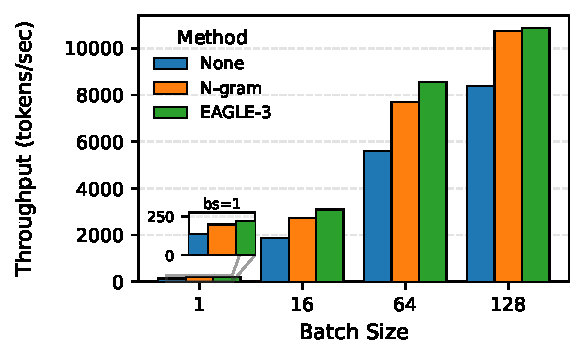
\includegraphics[width=\linewidth]{figures/e2e/thinking_qwen-8b-thinking_instructcoder.pdf}
\caption{Qwen3-8B-Thinking, InstructCoder}
\end{subfigure}

\begin{subfigure}[t]{0.22\textwidth}
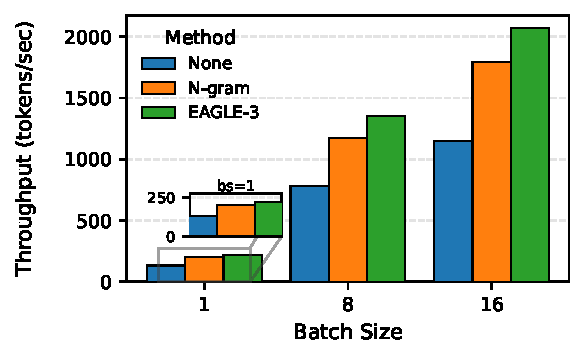
\includegraphics[width=\linewidth]{figures/e2e/thinking_qwen-8b-thinking_aime.pdf}
\caption{Qwen3-8B-Thinking, AIME22-24}
\end{subfigure}
\begin{subfigure}[t]{0.22\textwidth}
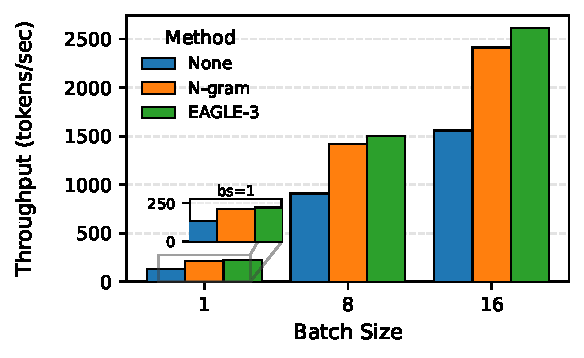
\includegraphics[width=\linewidth]{figures/e2e/thinking_qwen-8b-thinking-gpqa_gpqa_main.pdf}
\caption{Qwen3-8B-Thinking, GPQA-Main}
\end{subfigure}
\begin{subfigure}[t]{0.22\textwidth}
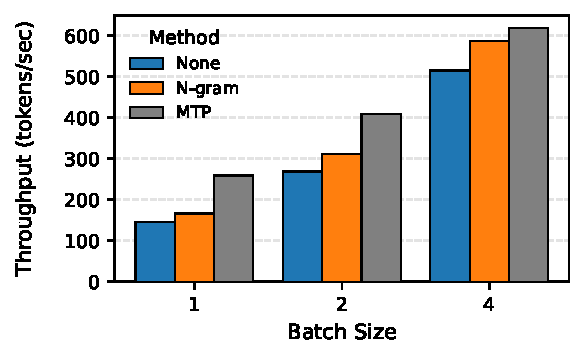
\includegraphics[width=\linewidth]{figures/e2e/thinking_glm4.5_aime.pdf}
\caption{GLM-4.5-Air, AIME22-24}
\end{subfigure}
\begin{subfigure}[t]{0.22\textwidth}
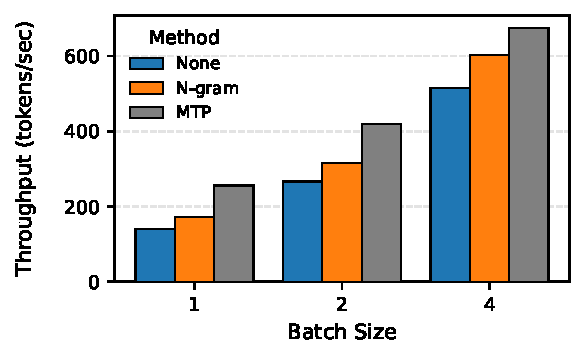
\includegraphics[width=\linewidth]{figures/e2e/thinking_glm4.5_gpqa_main.pdf}
\caption{GLM-4.5-Air, GPQA-Main}
\end{subfigure}
\caption{End-to-end performance on reasoning workloads. }
\label{fig:e2e-reasoning}
\end{center}
\end{figure*}

\begin{quoting}[leftmargin=1.5em, rightmargin=1.5em, vskip=0pt]
\textbf{Reasoning Workloads.}
\emph{Models and drafting methods that sustain high acceptance rates over long contexts—such as EAGLE-3 and, in some cases, $n$-gram—derive the greatest benefit on reasoning tasks. In contrast, MTP performance is limited by the reuse of a single MTP head across drafted tokens.}
\end{quoting}

As reasoning workloads become increasingly prevalent, understanding the effectiveness of speculative decoding (SD) in this regime becomes important. These workloads feature short prompts but long generation sequences. We evaluate SD on two representative reasoning benchmarks, AIME22–24~\cite{AIME-HF} and GPQA-Main~\cite{rein2023gpqagraduatelevelgoogleproofqa}.

As shown in \autoref{fig:e2e-reasoning}, we report the absolute generation throughput across different batch sizes. To ensure fair and consistent comparisons, we restrict our evaluation to medium batch sizes. Reasoning tasks typically involve long generation sequences, which can trigger request preemption once the KV cache becomes full. By avoiding such preemption, the reported results more accurately reflect the inherent efficiency of speculative decoding rather than performance artifacts caused by memory pressure.

For Qwen3-8B-Thinking, EAGLE-3 consistently leads across datasets, achieving 1.64$\times$--1.80$\times$ speedup over on GPQA-Main and AIME22–24, whereas $n$-gram performs comparably at 1.50$\times$--1.58$\times$. This trend likely arises because the model produces longer contexts and repetitive symbolic patterns, increasing opportunities for reuse. As shown later in~\autoref{sec:acc-behavior}, the average acceptance length in GPQA-Main generally grows with sequence length, with $n$-gram’s acceptance rising faster than EAGLE-3’s.

For GLM-4.5-Air, MTP outperforms $n$-gram but falls short of the theoretical upper bound, achieving 1.3$\times$--1.8$\times$ speedup on GPQA-Main. This gap is likely because the released open-source weights include only the first MTP module, which is trained primarily to predict the first token accurately but reused autoregressively for subsequent ones. Consequently, its position-wise acceptance rate (\(0.92 \rightarrow 0.68 \rightarrow 0.38\) on GPQA-Main), accuracy declines sharply across drafted tokens, shrinking the acceptance rate and thereby constraining the achievable speedup.


